\documentclass[10pt]{article} 
\usepackage[spanish]{babel}
\usepackage[utf8]{inputenc} 
\usepackage[left=1.50cm, right=1.50cm, top=1.50cm, bottom=1.50cm]{geometry}
\usepackage{blindtext}
\usepackage{multicol}
\usepackage{graphicx}
\usepackage{amsmath}
\usepackage{listings}
\usepackage{xcolor}

\title{Métodos de integración numérica}
\author{Gustavo Ramos}
\date{9 de Enero 2024}

\definecolor{codegreen}{rgb}{0,0.6,0} 
\definecolor{codegray}{rgb}{0.5,0.5,0.5}
\definecolor{codepurple}{rgb}{0.58,0,0.82} \definecolor{backcolour}{rgb}{0.95,0.95,0.92} 
\lstdefinestyle{mystyle}
{ 
	backgroundcolor=\color{backcolour},
	commentstyle=\color{codegreen}, 
	keywordstyle=\color{magenta}, 
	numberstyle=\tiny\color{codegray}, 
	stringstyle=\color{codepurple}, 
	basicstyle=\ttfamily\footnotesize, 
	breakatwhitespace=true, 
	captionpos=b,  
	keepspaces=true, 
	numbersep=5pt, 
	showspaces=false, 
	showstringspaces=false, 
	showtabs=false, 
	tabsize=2 
} 
\lstset{style=mystyle}

\begin{document}
	\maketitle
	\begin{abstract}
		Este documento expone los métodos de integración numérica y su programación en el lenguaje c, así mismo, se expondrá una aplicación en física medica, dicha nos ayudara a ver que método es más efectivo a ciertos decimales correctos.
	\end{abstract}
	\newpage
	\tableofcontents
	\newpage
	\begin{multicols}{2}
		\section{Introducción}
		Derivar es por mucho, más fácil que integrar, y es que para algunas integrales, es imposible el obtener una función analítica, así que se recurre a métodos numéricos que nos darán aproximaciones que, sobre el papel, son malas, así que recurriremos a una computadora con mucha más potencia de lectura, escritura y cálculo que nuestro cerebro, para así, conseguir precisiones de hasta diecisiete (o mas) decimales correctos.
		\section{Antecedentes}
		El cálculo integral representa una técnica con la que la humanidad ha logrado colocar en una nueva perspectiva a áreas como la geometría y la aritmética. Los inicios del cálculo son ya bien conocidos, Newton y Leibniz desarrollaron por separado sus ideas sobre el cálculo en el siglo XVII. A sabiendas de que la derivada sería una operación, una operación inversa que debía desarrollarse, y así también se trataron las integrales, un concepto que definió mejor Leibniz que Newton. Varias técnicas diferentes se fueron desarrollando después. Las sumas de Riemann (por Bernhard Riemann, consistente en la división por rectángulos del área bajo la curva), la regla del trapecio (consistente en la unión de puntos y no en la división por rectángulos), la regla de Simpson y el método de Romberg son ejemplos que se tratarán en esta entrada, y que suponen aproximaciones a los resultados de las integrales definidas.
		\section{Metodología}
		\subsection{Métodos de integración numérica}
		\subsubsection{Integral}
		Si tenemos una función continua y acotada en un intervalo, se dice que la función es integrable y su integral esta definida como:
		$$\int_a^b f(x) dx=F(b)-F(a)$$
		Sin embargo, encontrar $F(x)$ algunas veces suele ser imposible por medios analíticos, así que recurrimos a los métodos numéricos por ordenador para conseguir una aproximación lo suficientemente buena (dependerá de los decimales correctos).
		\subsubsection{Sumas de Riemman} 
		Si tenemos una función integrable $f(x)$, entonces, podemos hacer particiones rectangulares, el área bajo la curva es igual a la suma del área de todos esos rectángulos, sin embargo, podemos construir esos rectángulos de dos maneras como se muestra en la siguiente imagen:\\
		\begin{center}
			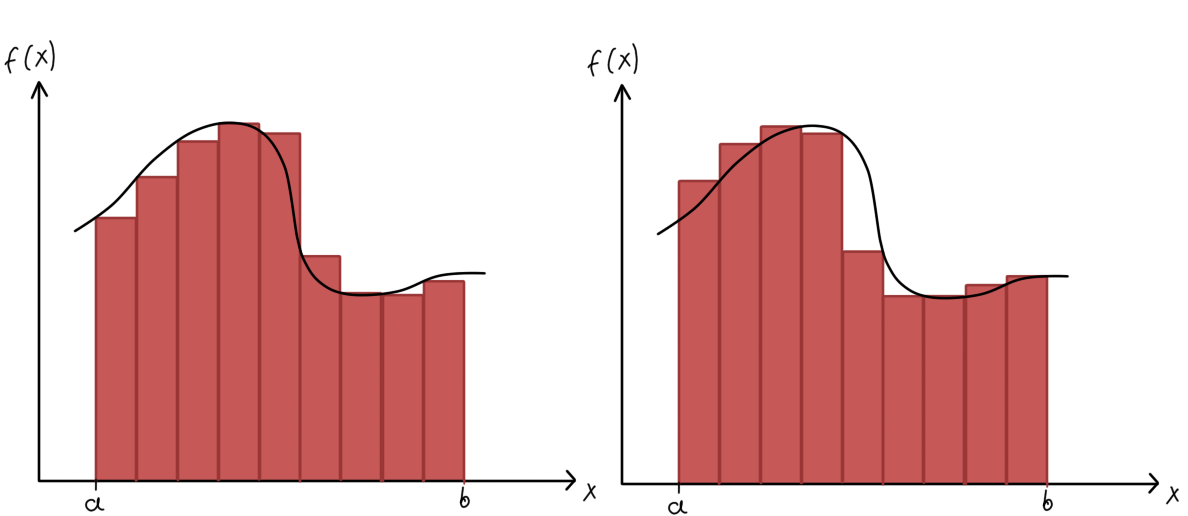
\includegraphics[scale=0.2]{../Imagenes/1.png}
		\end{center}
		Así, para $N$ particiones en un intervalo $(a,b)$, definimos las sumas de Riemman por la izquierda y por la derecha como:
		$$R_{izq}=\sum_{i=0}^{N-1}f(x_i)h$$
		$$R_{der}=\sum_{i=1}^{N}f(x_i)h$$
		donde h es la base de cada rectángulo, definida como:
		$$h=\frac{b-a}{N}$$
		y $x_i=a+ih$
		\subsubsection{Método de trapecio}
		Si a cada rectángulo le partimos la "cabeza", como se muestra en la imagen\\
		\begin{center}
			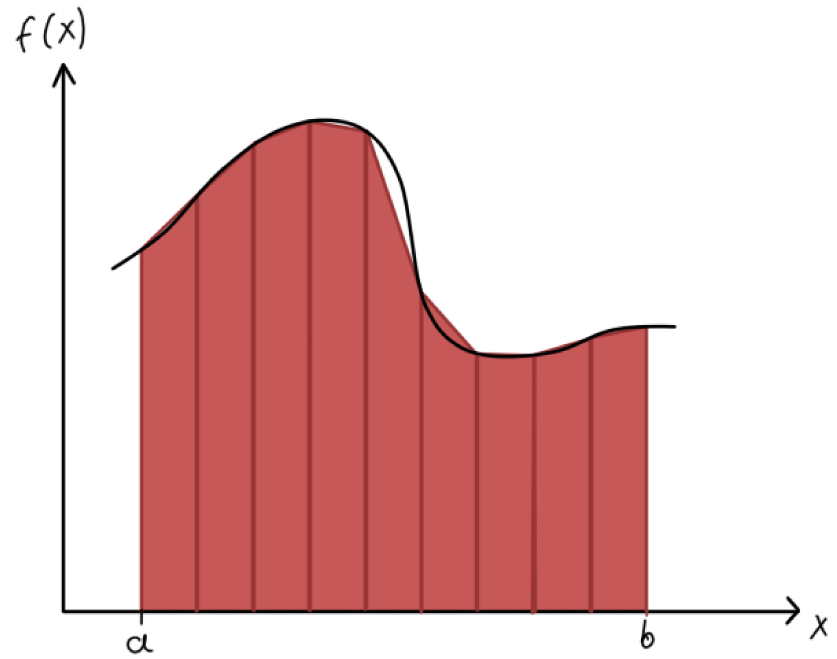
\includegraphics[scale=0.2]{../Imagenes/2.png}
		\end{center}
		Nos olvidamos de la suma por la izquierda y por la derecha, formando una sola suma, donde sumaremos el área de todos los trapecios formados, pero primero debemos de calcular el área de uno solo de estos trapecios.\\
		Podemos observar en la imagen que tenemos dos puntos y una linea recta, lo que significa un acomodo polinómico lineal, este acomodo esta definido como:
		$$f\left( a \right) + {{f\left( b \right) - f\left( a \right)} \over {b - a}}\left( {x - a} \right)$$
		Entonces, la integral la podemos aproximar como:
		$$A = \int_a^b {f\left( x \right)dx} \approx \left( {b - a} \right)\left[ {{{f\left( a \right) + f\left( b \right)} \over 2}} \right]$$
		Y si en lugar de hacer una sola división, hacemos $n$:
		$$A \approx  \frac{b - a}{2n}\left[ {{{f\left( a \right) + f\left( x_1 \right)}}}+{{{f\left( x_1 \right) + f\left( x_2 \right)}}}+\cdots \right]$$
		O lo que es igual:
		$$A\approx\frac{h}{2}\sum_{i=1}^{n}\left[ f(x_i)+f(x_{i+1}) \right]$$
				
		\subsubsection{Regla Simpson 1/3}
		Si en lugar de aproximar dos puntos a un ajuste lineal, ajustamos tres puntos a un polinomio de segundo grado en un rango $(a,b)$ como se muestra en la imagen:
		\begin{center}
			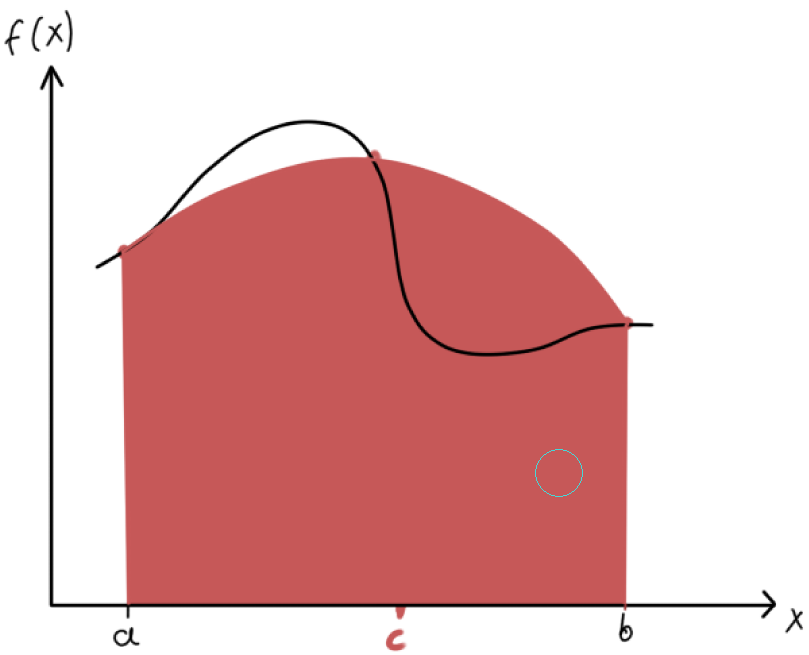
\includegraphics[scale=0.2]{../Imagenes/3.png}
		\end{center}
		La aproximación es mucho mejor, así pues, definimos los tres puntos, a primera aproximación: $(a,f(a))$, $(m,f(m)=f(b-a/2))$ y $(b,f(b))$, si hacemos la interpolación de Lagrange, tenemos que el polinomio es aproximadamente:
		$$f(x)\approx f(a){\frac {(x-m)(x-b)}{(a-m)(a-b)}}+f(m){\frac {(x-a)(x-b)}{(m-a)(m-b)}}$$
		$$+f(b){\frac {(x-a)(x-m)}{(b-a)(b-m)}}$$
		O, renombrando para simplificar los cálculos:
		$$f(x)\approx L_0(x)f(a)+L_1(x)f(m)+L_2(x)f(b)$$
		Donde podemos definir:
		$$I=\int_a^{a+2h}L_0(x)dx$$
		$$T=\int_a^{a+2h}L_1(x)dx$$
		$$Z=\int_a^{a+2h}L_2(x)dx$$
		Para el calculo de $I$, con $h=b-c=c-a=(b-a)/2$ tenemos que:
		\begin{equation*}
			\begin{split}
				I&=\int_a^{a+2h}L_0(x) dx \\
				 &=\frac{1}{2h^2}\int_a^{a+2h}(x-(a+h))(x-(a+2h))dx
			\end{split}
		\end{equation*}
		Haciendo un cambio de variable $u=x-a-h$
		\begin{equation*}
			\begin{split}
				I&=\frac{1}{2h^2}\int_{-h}^h u(u-h)du\\
				 &=\frac{1}{2h^2}\int_{-h}^h u^2-uh du\\
				 &=\frac{h}{3}
			\end{split}
		\end{equation*}
		Para las otras dos constantes, $I=Z$ y $T=4h/3$, así, podemos aproximar el área como:
		$$A\approx \frac{h}{3}\left[ f(a)+4f(c)+f(b) \right]$$
		Y si en lugar de tomar dos puntos, tomamos n, haciendo particiones de tres en tres, tenemos:
		\begin{equation*}
			\begin{split}
				A\approx \frac{h}{3}[ f(x_0)+4f(x_1)+f(x_2)&+f(x_2)+\\
				&+4f(x_3)+f(x_4)+\cdots]
			\end{split}
		\end{equation*}
		Agrupando términos, podemos dividir en dos sumas:
		$$A\approx \frac {h}{3}\left[f(x_{0})+2\sum _{j=1}^{{\frac {n}{2}}-1}f(x_{2j})+4\sum _{j=1}^{\frac {n}{2}}f(x_{2j-1})+f(x_{n})\right]$$
		Por lo que $n$ tiene que ser un numero par. 
		
		\subsubsection{Regla Simpson 3/8}
		Si en lugar de aproximar a una parábola, aproximamos a una curva cubica en un rango $(x_0=a,x_3=b)$ con $x_i=a+ih$, $h=(x_3-x_0)/3=x_{i}-x_{i-1}$ como vemos en la imagen:
		\begin{center}
			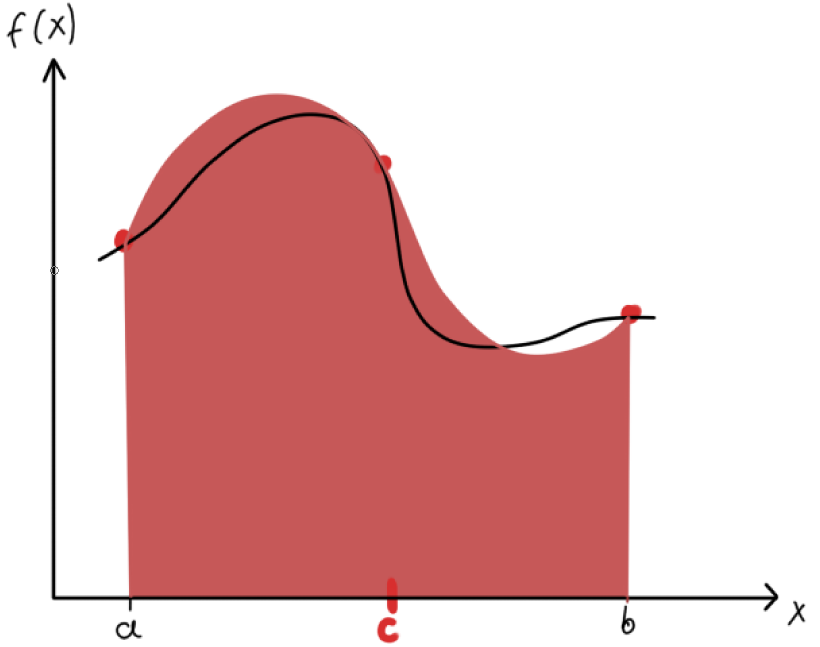
\includegraphics[scale=0.2]{../Imagenes/4.png}
		\end{center}
		Y aplicando nuevamente la aproximación de lagrange para cuatro puntos $(x_0,f(x_0))$, $(x_1,f(x_1))$, $(x_2,f(x_2))$, $(x_3,f(x_3))$:
		\begin{equation*}
			\begin{split}
				 f(x)\approx &f(x_0)\frac{(x-x_1)(x-x_3)(x-x_3)}{(x_0-x_1)(x_0-x_2)(x_0-x_3)}+\\ &f(x_1)\frac{(x-x_0)(x-x_2)(x-x_3)}{(x_1-x_0)(x_1-x_2)(x_1-x_3)}+\\
				 &f(x_2)\frac{(x-x_0)(x-x_1)(x-x_3)}{(x_2-x_0)(x_2-x_1)(x_2-x_3)}+\\ &f(x_3)\frac{(x-x_0)(x-x_1)(x-x_2)} {(x_3-x_0)(x_3-x_1)(x_3-x_2)}
			\end{split}
		\end{equation*}
		Que para simplificar, lo podemos reescribir como:
		$$f(x)\approx L_0(x)f(x_0)+L_1(x)f(x_1)+L_2(x)f(x_2)+L_3(x)f(x_3)$$
		Y definimos las constantes:
		$$I=\int_{x_0}^{x_3} L_0(x)dx$$
		$$T=\int_{x_0}^{x_3} L_1(x)dx$$
		$$Z=\int_{x_0}^{x_3} L_2(x)dx$$
		$$E=\int_{x_0}^{x_3} L_3(x)dx$$
		Constantes que, podemos calcular fácilmente, $I=E=3h/8$ y $T=Z=9h/8$, así, podemos aproximar el área como:
		$$A\approx {\frac {3h}{8}}\left[f(x_0)+3f\left({x_1}\right)+3f\left({x_2}\right)+f(x_3)\right]$$
		Y si en lugar de hacer esto una sola vez, lo hacemos $n$ veces:
		\begin{equation*}
			\begin{split}
				A\approx \frac{3h}{8}\left[f(x_0)+3f(x_1)+3f(x_2)+f(x_3)+\right.\\
				\left. +f(x_3)+3f(x_4)+3f(x_5)+f(x_6)+\cdots \right]
			\end{split}
		\end{equation*}
		Si lo agrupamos en tres sumas, tenemos:
		\begin{equation*}
			\begin{split}
				\frac{3h}{8} \left[f(x_0) + 3\sum_{i=0}^{\frac{n}{3}-1}f(x_{3i+1}) +3\sum_{i=0}^{\frac{n}{3}-1}f(x_{3i+2})+\right. \\
				\left.+2\sum_{i=0}^{\frac{n}{3}-2}f(x_{3i+3}) + f(x_n)\right] 
			\end{split}
		\end{equation*}
		Por lo que $n$ tiene que ser un múltiplo de 3.
		\subsection{Aplicación biomédica: Administración de solución salina por vía intravenosa}
		Durante una intervención quirúrgica, los pacientes suelen
		requerir la administración de líquidos por vía intravenosa para
		mantener una presión arterial adecuada. Consideremos una
		bolsa cilíndrica que contiene la solución salina de
		NaCl que se suministra al paciente. Por simplificación, se
		considerará que el líquido fluye por efecto de la gravedad por
		un agujero situado en la parte inferior de la bolsa y se introduce
		posteriormente en el flujo sanguíneo del paciente. La única
		resistencia presente al movimiento de la solución es la
		resistencia del tubo, la cual determina el tiempo que tarda la
		bolsa en vaciarse. \\
		Para calcularlo se planteará un equilibrio cinemático calculado
		mediante la ecuación de Bernouilli, pero teniendo en cuenta la fricción existente en
		el tubo: la energía a la altura del fluido en la bolsa será igual a la energía del líquido
		saliendo del tubo menos la pérdida por fricción a lo largo del mismo. La altura del
		fluido en la bolsa con respecto al paciente es, a la vista de la figura, $(z+L)$ cm.
		La presión en el interior del tubo debido a la fricción con las paredes viene dada por la ecuación de Hagen-Poisseuille:
		$$\Delta P=\frac{8QL\mu}{\pi R_{tubo}^4}=\frac{32vL\mu}{d^2}$$
		donde $Q$ es el flujo (caudal) del fluido, $d$ es el diámetro interno del tubo, $\Delta P$ es la caída de presión entre los dos extremos, $\mu$ es la viscosidad dinámica, $L$ la longitud del tubo a lo largo del eje $z$ y $v$ es la velocidad del fluido a la salida del tubo.
		La ecuación de Bernouilli en este problema es la siguiente:
		$$g(z+L)=\frac{v^2}{2}+\frac{\Delta P}{\rho}=\frac{v^2}{2}+\frac{32vL\mu}{d^2\rho}$$
		donde $\Delta P/\rho$ es el termino de perdida de energía debido a la fricción.
		Despejando $\mu$ y considerando $\alpha=64L\mu/d^2\rho$ y resolviendo la ecuación de segundo grado:
		$$v=\frac{-\alpha+\sqrt{\alpha^2+8g(z+L)}}{2}$$
		Como el flujo de fluido en la bolsa es igual al del tubo:
		$$-\rho\pi R_{bolsa}^2\frac{dz}{dt}=\rho\pi\frac{d^2}{4}v$$
		Reordenando y sustituyendo $Q$ obtenemos finalmente:
		$$dt=-4\frac{R_{bolsa}^2}{d^2v}dz=-\frac{8R_{bolsa}^2}{(-\alpha+\sqrt{\alpha^2+8g(z+L)})d^2}dz$$			
		\section{Análisis y resultados}
		\subsubsection{Condiciones del problema a resolver}
		Recordando la anterior función, tenemos que:
		$$t=\frac{8R_{bolsa}^2}{d^2}\int_a^b-\frac{1}{(-\alpha+\sqrt{\alpha^2+8g(z+L)})}dz$$
		La integración de esta función, de manera analítica, puede conllevar un trabajo intenso, pues su integral analítica lleva un logaritmo natural de por medio, así que se recurre a los métodos numéricos para encontrar un valor a ciertas condiciones.\\
		Consideremos que $L=91.44$ cm, $d=0.1$ cm, $R_{bolsa}=10$ cm, la viscosidad de la solución salina en $\mu=0.01$ Poise, la densidad $\rho=1$g/cm$^3$ y la gravedad $g=981$ cm/s$^2$, además, consideremos que queremos que se vacié el 90\%  del recipiente, así que el intervalo sera de $z=50$ hasta $z=5$, así que la integral se vuelve:
		$$t=\frac{8\cdot 10^2}{0.1^2}\int_{5}^{50}\frac{1}{(-\alpha+\sqrt{\alpha^2+8\cdot981 \cdot(z+91.44)})}dz$$
		\subsubsection{Resultados}
		En la siguiente tabla se muestran los resultados de la integral obtenidos en los cuatro programas a distintos números de pasos $n$:
		\begin{center}
		\begin{tabular}{| c | c | c |}
			\hline
			Método & $n=10$ & $n=20$ \\ \hline
			Riemman & Prom= $0.575093$ & Prom=$0.5749845$ \\
			Trapecio & $0.622192$ & $0.598714$\\
			Simpson 1/3 & $0.574948$ & $0.574948$ \\ 
			Simpson 3/8 & $0.525762$ & $0.526054$ \\ \hline
		\end{tabular}
		\end{center}
		\section{Conclusiones}
		El articulo original nos establece un valor exacto de la integral en $0.5749481$, así, guiándonos con este valor, vemos que el método de Simpson 1/3 es el más eficiente, el método de sumas de Riemman lo despreciamos completamente, pues obtenemos dos valores que hay que promediar, lo que no se tiene que hacer con el resto de procedimientos, en este caso parece ser que el método del Trapecio no funciona como se esperaría, después de este, el método de Simpson 3/8 es el segundo peor, a pesar del numero de particiones, da un valor con solo un decimal de precisión.
	\end{multicols}
	\appendix 
	\section{Diseño del codigo} 
		\subsection{Programa principal}
			\lstinputlisting[language=c]{../main.c}
		\subsection{Cabecera}
			\lstinputlisting[language=c]{../Metodos.h}
	\begin{multicols}{2} 
		\section{Referencias} 
			$[1]$ Chapra, S. C., \& Canale, R. P. (2011). Métodos Numéricos para Ingenieros. Ciudad de México: McGraw-Hil \\
			
			$[2]$ Epperson, J. and Epperson, J., 2013. Solutions manual to accompany An introduction to numerical methods and Analysis, Second edition. 2nd ed. Hoboken, N.J: Wiley. \\
			
			$[3]$ Khan Academy. (2015). Obtenido de:\\ https://es.khanacademy.org/math/integral-calculus/solid-revolution-topic\\
	\end{multicols} 
\end{document}